% rubber: set program xelatex
%%%%%%%%%%%%%%%%%%%%%%%%%%%%%%%%%%%%%%%
% Deedy - One Page Two Column Resume
% LaTeX Template
% Version 1.2 (16/9/2014)
%
% Original author:
% Debarghya Das (http://debarghyadas.com)
%
% Original repository:
% https://github.com/deedydas/Deedy-Resume
%
% IMPORTANT: THIS TEMPLATE NEEDS TO BE COMPILED WITH XeLaTeX
%
% This template uses several fonts not included with Windows/Linux by
% default. If you get compilation errors saying a font is missing, find the line
% on which the font is used and either change it to a font included with your
% operating system or comment the line out to use the default font.
% 
%%%%%%%%%%%%%%%%%%%%%%%%%%%%%%%%%%%%%%
% 
% TODO:
% 1. Integrate biber/bibtex for article citation under publications.
% 2. Figure out a smoother way for the document to flow onto the next page.
% 3. Add styling information for a "Projects/Hacks" section.
% 4. Add location/address information
% 5. Merge OpenFont and MacFonts as a single sty with options.
% 
%%%%%%%%%%%%%%%%%%%%%%%%%%%%%%%%%%%%%%
%
% CHANGELOG:
% v1.1:
% 1. Fixed several compilation bugs with \renewcommand
% 2. Got Open-source fonts (Windows/Linux support)
% 3. Added Last Updated
% 4. Move Title styling into .sty
% 5. Commented .sty file.
%
%%%%%%%%%%%%%%%%%%%%%%%%%%%%%%%%%%%%%%%
%
% Known Issues:
% 1. Overflows onto second page if any column's contents are more than the
% vertical limit
% 2. Hacky space on the first bullet point on the second column.
%
%%%%%%%%%%%%%%%%%%%%%%%%%%%%%%%%%%%%%%


\documentclass[]{deedy-resume-openfont}
\usepackage{fancyhdr}

\usepackage[dvips,xetex]{graphicx}
% \usepackage{ifpdf,mla}
 
\pagestyle{fancy}
\fancyhf{}
 
\begin{document}

%%%%%%%%%%%%%%%%%%%%%%%%%%%%%%%%%%%%%%
%
%     LAST UPDATED DATE
%
%%%%%%%%%%%%%%%%%%%%%%%%%%%%%%%%%%%%%%
\lastupdated

%%%%%%%%%%%%%%%%%%%%%%%%%%%%%%%%%%%%%%
%
%     TITLE NAME
%
%%%%%%%%%%%%%%%%%%%%%%%%%%%%%%%%%%%%%%
\namesection{Stefan}{Matting}{
    \href{mailto:stefan.matting@gmail.com.com}{stefan.matting@gmail.com} | +4917625558115
    % \urlstyle{same}\href{http://debarghyadas.com}{debarghyadas.com}| \href{http://fb.co/dd}{fb.co/dd}\\
    % \href{mailto:deedy@fb.com}{deedy@fb.com} | 607.379.5733 | \href{mailto:dd367@cornell.edu}{dd367@cornell.edu}
}

%%%%%%%%%%%%%%%%%%%%%%%%%%%%%%%%%%%%%%
%
%     COLUMN ONE
%
%%%%%%%%%%%%%%%%%%%%%%%%%%%%%%%%%%%%%%

\begin{minipage}[t]{0.33\textwidth} 

%%%%%%%%%%%%%%%%%%%%%%%%%%%%%%%%%%%%%%
%     LINKS
%%%%%%%%%%%%%%%%%%%%%%%%%%%%%%%%%%%%%%


\section{About} 

\begin{center}
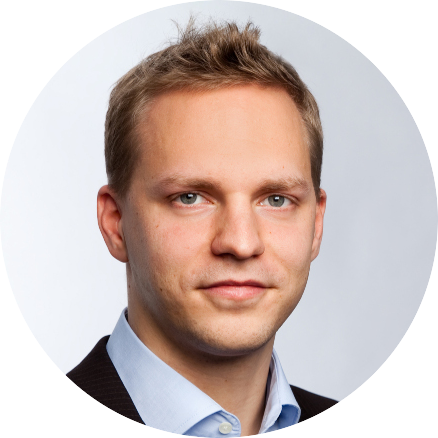
\includegraphics[scale=0.3]{mug-round.png}
\end{center}

Github: \href{https://github.com/smatting}{\bf smatting} \\
LinkedIn:  \href{https://www.linkedin.com/in/stefanmatting/}{\bf stefanmatting} \\
Hobbies: making \& listing to music \textbullet{} programming \textbullet{} running

%%%%%%%%%%%%%%%%%%%%%%%%%%%%%%%%%%%%%%
%     SKILLS
%%%%%%%%%%%%%%%%%%%%%%%%%%%%%%%%%%%%%%



\sectionsep
\section{Skills}

\subsection{Programming}
    Python \textbullet{}
    SQL \textbullet{}
    C/C++ \textbullet{}
    Mathematica \textbullet{}
    Matlab \textbullet{}
    Java \textbullet{}
    Javascript \textbullet{}
    Clojure \textbullet{}
    Haskell 

\sectionsep
\subsection{Data Science}
Data Wrangling \& Analysis (Python data tools) \textbullet{}
Machine Learning (scikit-learn, xgboost) \textbullet{}
Deep Learning (tensorflow, theano) \textbullet{}
Bayesian Statistics (PyMC3, edward)
   
\sectionsep
\subsection{Data Products}
Data Services (gunicorn, nginx, RabbitMQ, Docker) \textbullet{}
DBs (Postgresql, Elasticsearch, MongoDB)


%%%%%%%%%%%%%%%%%%%%%%%%%%%%%%%%%%%%%%
%
%     COLUMN TWO
%
%%%%%%%%%%%%%%%%%%%%%%%%%%%%%%%%%%%%%%

\end{minipage} 
\hfill
\begin{minipage}[t]{0.62\textwidth} 

%%%%%%%%%%%%%%%%%%%%%%%%%%%%%%%%%%%%%%
%     EXPERIENCE
%%%%%%%%%%%%%%%%%%%%%%%%%%%%%%%%%%%%%%

\section{Experience}

\runsubsection{Outfittery GmbH}
\descript{| Machine Learning Specialist }
\location{Dec 2013 - Present | Berlin}
\vspace{12pt} % Hacky fix for awkward extra vertical space
\begin{tightemize}
\item Hired as the first data scientist and helped building the data department for over 3 years
\item Build the platform that integrates all algorithms into the IT system
\item Fashion article recommendation based on Matrix Factorization and Deep Learning
\item Optimized several business processes with A/B-testing and ML models
\item Developed a business forecast model based on a Markov chain model
\item Estimated customer behaviour with various ML models
\item Visual similarity of fashion items with convolutional neural nets
\item Migrated all customer and article data between systems
\item Lead a small team of data scientists
\end{tightemize}
\sectionsep


\runsubsection{Fraunhofer-Institut für Solare Energiesysteme}
\descript{| Research assistant }
\location{Mar 2008 - Feb 2013 | Freiburg im Breisgau}
\begin{tightemize}
\item Research assistant to Dr. Simon Schwunk
\item Developed a modular simulation software for photovoltaic systems in C++.
\item Assisted in developing algorithms that estimate that internal state of several battery types . TODO: ref to patent
\item Ported multiple algorithms to embedded systems in C
\end{tightemize}
\sectionsep


\runsubsection{Universitäts-Klinikum Freiburg}
\descript{| Research assistant }
\location{Jun 2010 - Nov 2010 | Freiburg im Breisgau}
\begin{tightemize}
\item Research assistant to Prof. Dr. Thilo Hinterberger
\item Assisted in developing software system that evaluates EEG measurements in C++.
\end{tightemize}
\sectionsep

%%%%%%%%%%%%%%%%%%%%%%%%%%%%%%%%%%%%%%
%     EDUCATION
%%%%%%%%%%%%%%%%%%%%%%%%%%%%%%%%%%%%%%

\section{Education} 

\subsection{Albert-Ludwigs-Universität Freiburg}
\descript{Diplom Mathematik}
\location{Sep 2013 | Freiburg \\
    Final grade: 1.0}
\sectionsep
Coursework:
\begin{tightemize}
\item random trees
\end{tightemize}
\sectionsep

\subsection{Robert-Bosch Gymnasium}
\location{Jul 1994 | Wendlingen, BW}
\sectionsep

%%%%%%%%%%%%%%%%%%%%%%%%%%%%%%%%%%%%%%
%     COURSEWORK
%%%%%%%%%%%%%%%%%%%%%%%%%%%%%%%%%%%%%%

% \section{Coursework}
% \subsection{Graduate}
% Advanced Machine Learning \\
% Open Source Software Engineering \\
% Advanced Interactive Graphics \\
% Compilers + Practicum \\
% Cloud Computing \\
% Evolutionary Computation \\
% Defending Computer Networks \\
% Machine Learning \\
% \sectionsep

% \subsection{Undergraduate}
% Information Retrieval \\
% Operating Systems \\
% Artificial Intelligence + Practicum \\
% Functional Programming \\
% Computer Graphics + Practicum \\
% {\footnotesize \textit{\textbf{(Research Asst. \& Teaching Asst 2x) }}} \\
% Unix Tools and Scripting \\


%%%%%%%%%%%%%%%%%%%%%%%%%%%%%%%%%%%%%%
%     RESEARCH
%%%%%%%%%%%%%%%%%%%%%%%%%%%%%%%%%%%%%%

% \section{Research}
% \runsubsection{Cornell Robot Learning Lab}
% \descript{| Researcher}
% \location{Jan 2014 – Jan 2015 | Ithaca, NY}
% Worked with \textbf{\href{http://www.cs.cornell.edu/~ashesh/}{Ashesh Jain}} and \textbf{\href{http://www.cs.cornell.edu/~asaxena/}{Prof Ashutosh Saxena}} to create \textbf{PlanIt}, a tool which  learns from large scale user preference feedback to plan robot trajectories in human environments.  
% \sectionsep

% \runsubsection{Cornell Phonetics Lab}
% \descript{| Head Undergraduate Researcher}
% \location{Mar 2012 – May 2013 | Ithaca, NY}
% Led the development of \textbf{QuickTongue}, the first ever breakthrough tongue-controlled game with \textbf{\href{http://conf.ling.cornell.edu/~tilsen/}{Prof Sam Tilsen}} to aid in Linguistics research. 
% \sectionsep

%%%%%%%%%%%%%%%%%%%%%%%%%%%%%%%%%%%%%%
%     AWARDS
%%%%%%%%%%%%%%%%%%%%%%%%%%%%%%%%%%%%%%

% \section{Awards} 
% \begin{tabular}{rll}
% 2014	     & top 52/2500  & KPCB Engineering Fellow\\
% 2014	     & 1\textsuperscript{st}/50  & Microsoft Coding Competition, Cornell\\
% 2013	     & National  & Jump Trading Challenge Finalist\\
% 2013     & 7\textsuperscript{th}/120 & CS 3410 Cache Race Bot Tournament  \\
% 2012     & 2\textsuperscript{nd}/150 & CS 3110 Biannual Intra-Class Bot Tournament \\
% 2011     & National & Indian National Mathematics Olympiad (INMO) Finalist \\
% \end{tabular}
% \sectionsep

%%%%%%%%%%%%%%%%%%%%%%%%%%%%%%%%%%%%%%
%     PUBLICATIONS
%%%%%%%%%%%%%%%%%%%%%%%%%%%%%%%%%%%%%%

% \section{Publications} 
% \renewcommand\refname{\vskip -1.5cm} % Couldn't get this working from the .cls file
% \bibliographystyle{abbrv}
% \bibliography{publications}
% \nocite{*}

\end{minipage} 
\end{document}  \documentclass[]{article}
